\section{Neural Retrieval Models}
\subsection{Distributed Word Representations}
\begin{itemize}
	\item Latent, dense vector representation to model semantic similarity/relations
	
\end{itemize}
\subsubsection{Skip-gram}
\begin{itemize}
	\item \textbf{Skip gram}: learn to predict neighboring words in a small context window
	\item Model probability by similarity between word and context vectors (two matrices):
	$$p(w_k|w_j) = \frac{\exp\left(c_k \cdot v_j\right)}{\sum_{i\in|V|}} \exp\left(c_i \cdot v_j\right)$$
	\item Denominator can be computationally expensive if vocabulary is quite large. Thus, we can approximate it by taking just a few negative examples $\implies$ negative sampling
	\item Overall, skip gram will learn two representations for each word (context $C$ and target words $V$) from which me most likely only use $V$ (visualized in Figure~\ref{img:neural_ir_skip_gram})
	\begin{figure}[ht]
		\centering
		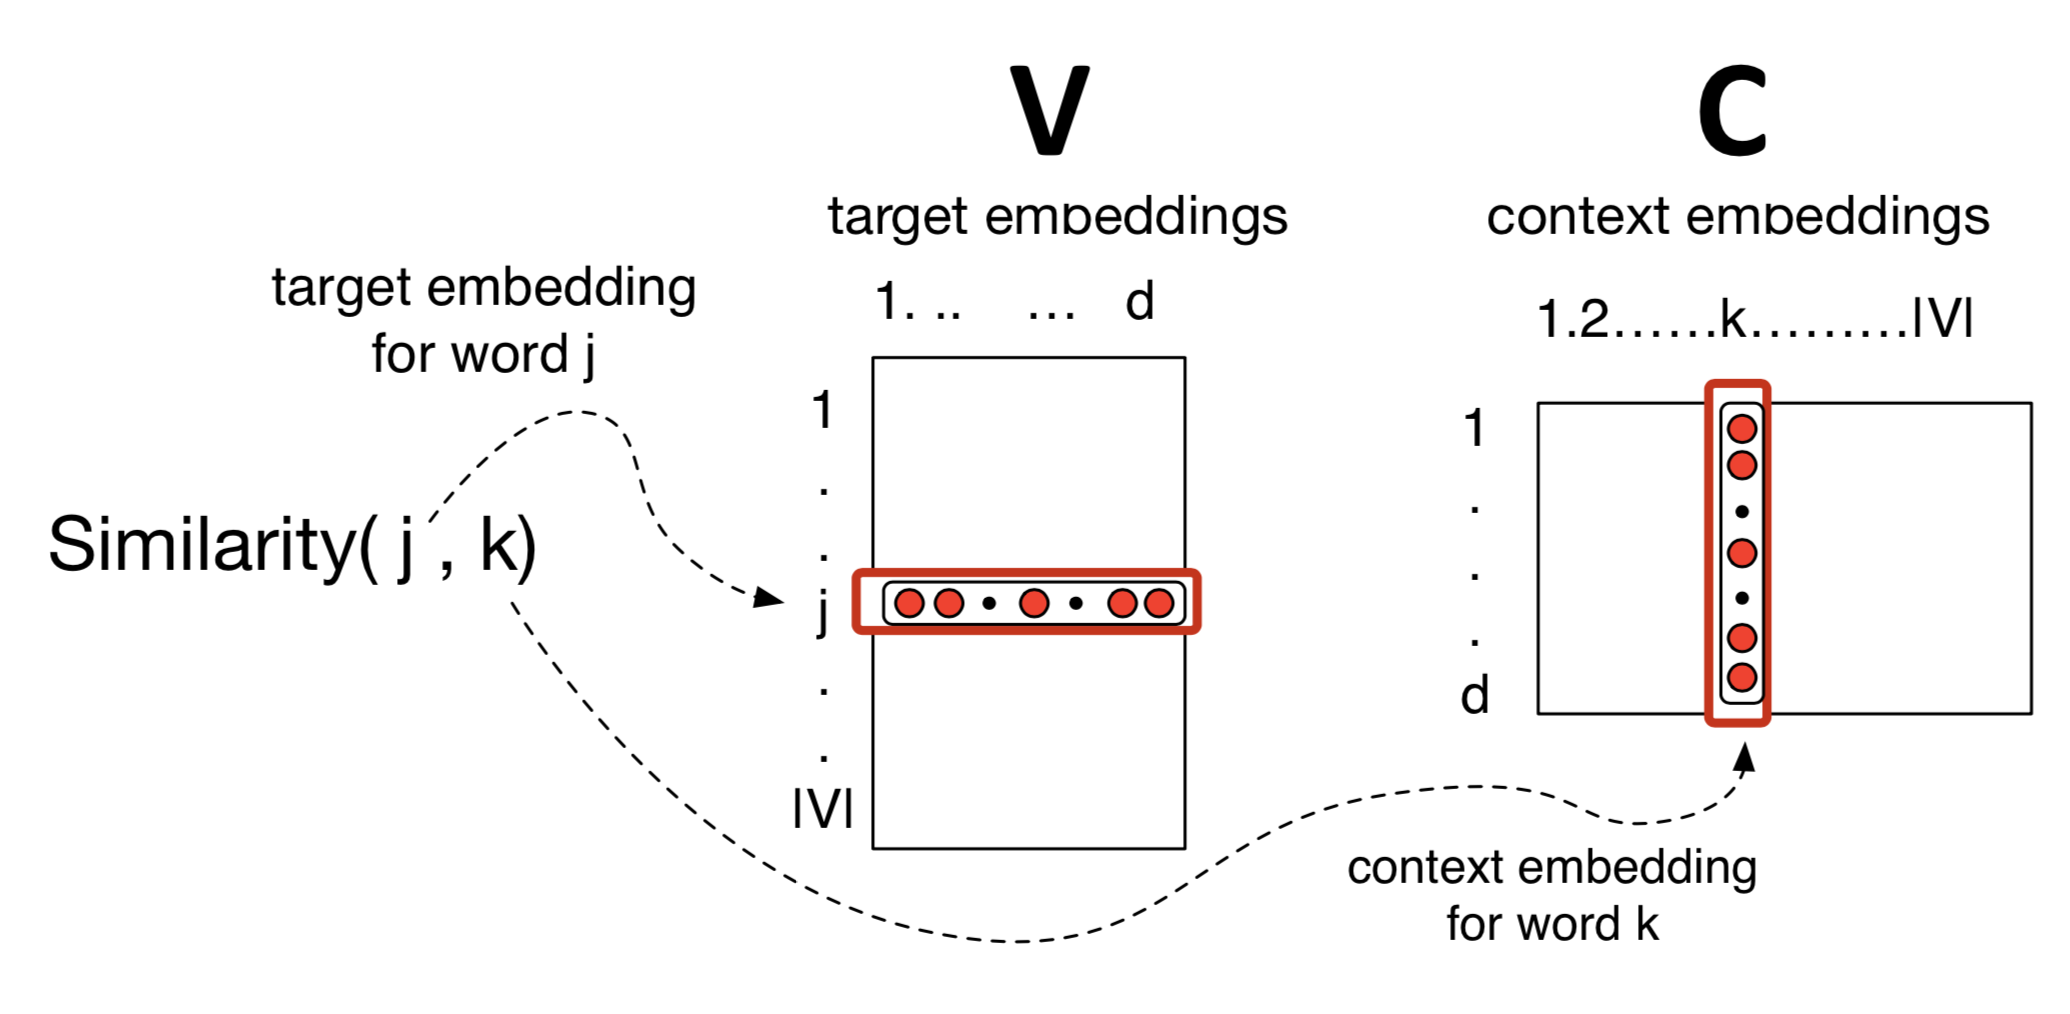
\includegraphics[width=0.4\textwidth]{figures/neural_ir_skip_gram.png}
		\caption{Visualization of skip gram method for learning word representations}
		\label{img:neural_ir_skip_gram}
	\end{figure}
	\item Skip gram shows to capture relational meaning (\texttt{KING - MAN + WOMAN = QUEEN})
\end{itemize}
\subsubsection{Using word embeddings in IR}
\begin{itemize}
	\item \textbf{Generalized Language Model}
	\begin{itemize}
		\item The standard language model assume that a term $t_q$ occurring in $q$ is being sampled from a document or a background collection (smoothing):
		$$p_{LM}(t_q|d) = \lambda \cdot p(t_q|d) + (1 - \lambda) \cdot p(t_q|C)$$
		\item The generalized language model extends this idea by also considering terms that are similar to $t_q$ (for example synonyms):
		$$p_{LM}(t_q|d) = \lambda \cdot p(t_q|d) + \alpha \sum\limits_{t'\in d} p(t_q|t',d) p(t'|d) + \beta \sum\limits_{t' \in N_t} p(t_q|t',C) p(t'|C) + (1 - \alpha - \beta - \lambda) \cdot p(t_q|C)$$
		where $$p(t_q|t',d) = \frac{sim(t',t_q)}{\sum_{t''\in d} sim(t',t'')} \text{\hspace{2mm}and\hspace{2mm}} p(t'|d) = \frac{tf(t';d)}{|d|}$$
		$N_t$ is the set of the most similar words to $t_q$.
	\end{itemize}
	\item \textbf{Word Mover's distance}
	\begin{itemize}
		\item For every word $w_i$ in the query $q$, look for the word with the highest similarity/smallest distance in document $d$
		\item Score a document by the sum of the pairwise distances. The document with the smallest distance gets the highest rank
		\item However, this approach doesn't care about the whole document but only the best matches
	\end{itemize}
\end{itemize}
\subsection{Compositionality}
\begin{itemize}
	\item To match queries and documents in the embedding space, we need to combine the words in each $\implies$ compositionality
\end{itemize}
\subsubsection{Aggregate word vectors}
\begin{itemize}
	\item Apply simple rules/arithmetic to combine word vectors
	\item Example: \textbf{Dual Embedding Space Model} 
	\begin{itemize}
		\item represent a document by the centroid of its word vectors $\bm{\overline{D}} = \frac{1}{|D|}\sum_{\bm{d}_j \in D} \frac{\bm{d}_j}{||\bm{d}_j||}$
		\item The query-document similarity is the average over query words of cosine similarity:\\ $\text{DESM}(Q,D) = \frac{1}{|Q|}\sum_{q_i \in Q} \frac{\bm{q}_i^T \bm{\overline{D}}}{||\bm{q}_i|| \cdot ||\bm{\overline{D}}||}$
		\item We can also use both the IN (word) and OUT (context) embeddings from skip-gram to optimize matching. What worked best was using IN representations for the query and OUT for document
		\item In the ranking system, we either first rank documents by BM25 and rerank top $N$ with DESM, or use a linear combination of both scores
	\end{itemize}
\end{itemize}
\subsubsection{Tune and Aggregate word vectors}
\begin{itemize}
	\item Learn task-specific representations and not rely on pure skip-gram
	\item \textbf{Paragraph2vec}
	\begin{itemize}
		\item Generalizes word2vec to whole documents by embedding them in a fixed-size vector
		\item Two different approaches. First is \textit{distributed memory}:
		\begin{itemize}
			\item We are trying to predict the next word based on a few previous context word \textit{and} a paragraph embedding. 
			\item Both the word and paragraph embeddings are learned during this process
			\item Input embeddings can either be concatenated or averaged (commonly first one is applied)
			\item Visualization in Figure~\ref{img:neural_models_distributed_memory}
			\begin{figure}[ht]
				\centering
				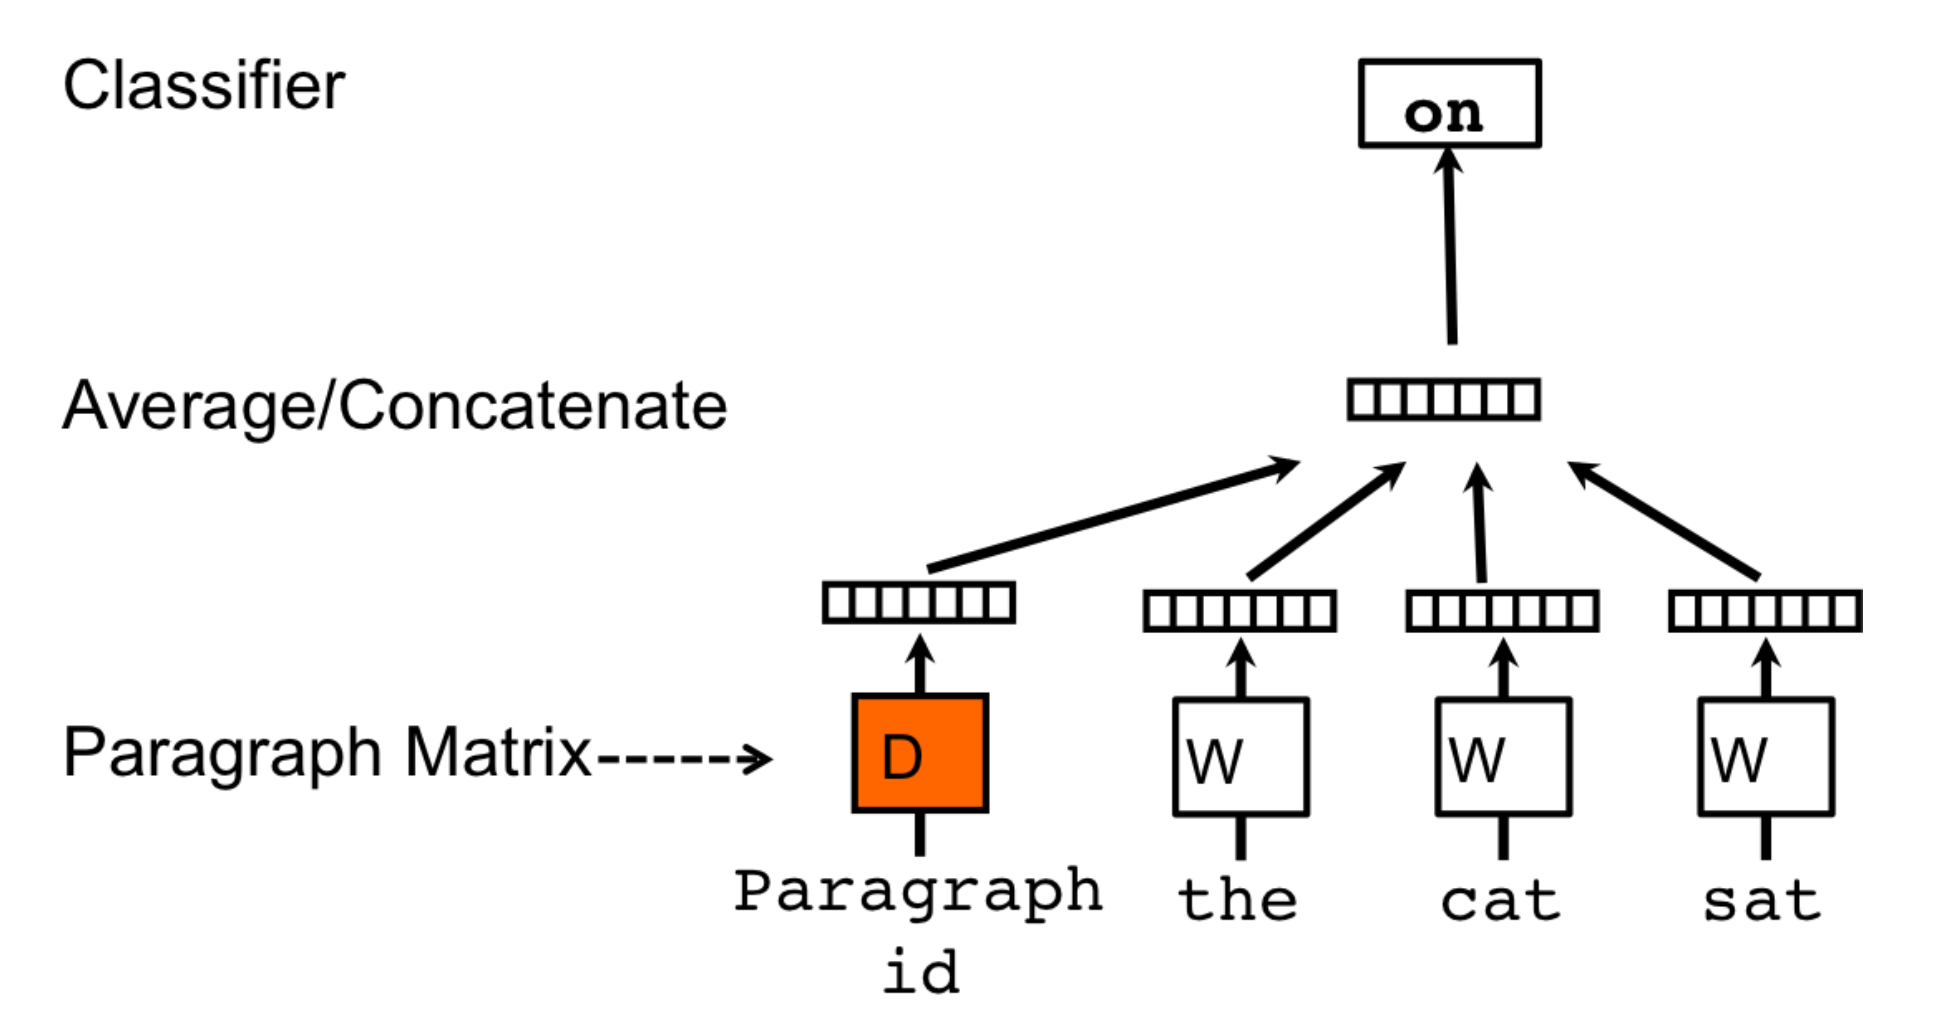
\includegraphics[width=0.3\textwidth]{figures/neural_models_distributed_memory.png}
				\caption{Distributed memory model. }
				\label{img:neural_models_distributed_memory}
			\end{figure}
		\end{itemize}
		\item Second method: \textit{Distributed bag of words}
		\begin{itemize}
			\item In this approach, we don't consider the context words but try to predict all possible words in the paragraph given the embedding vector
			\item This is done by sampling a random word at every SGD iteration from the small text windows, and train the classifier on predicting this word
			\item Thus, we optimize the embedding regarding representing the word distribution in the paragraph
			\item The distributed BOW is visualized in Figure~\ref{img:neural_model_distributed_BOW}
			\begin{figure}[ht]
				\centering
				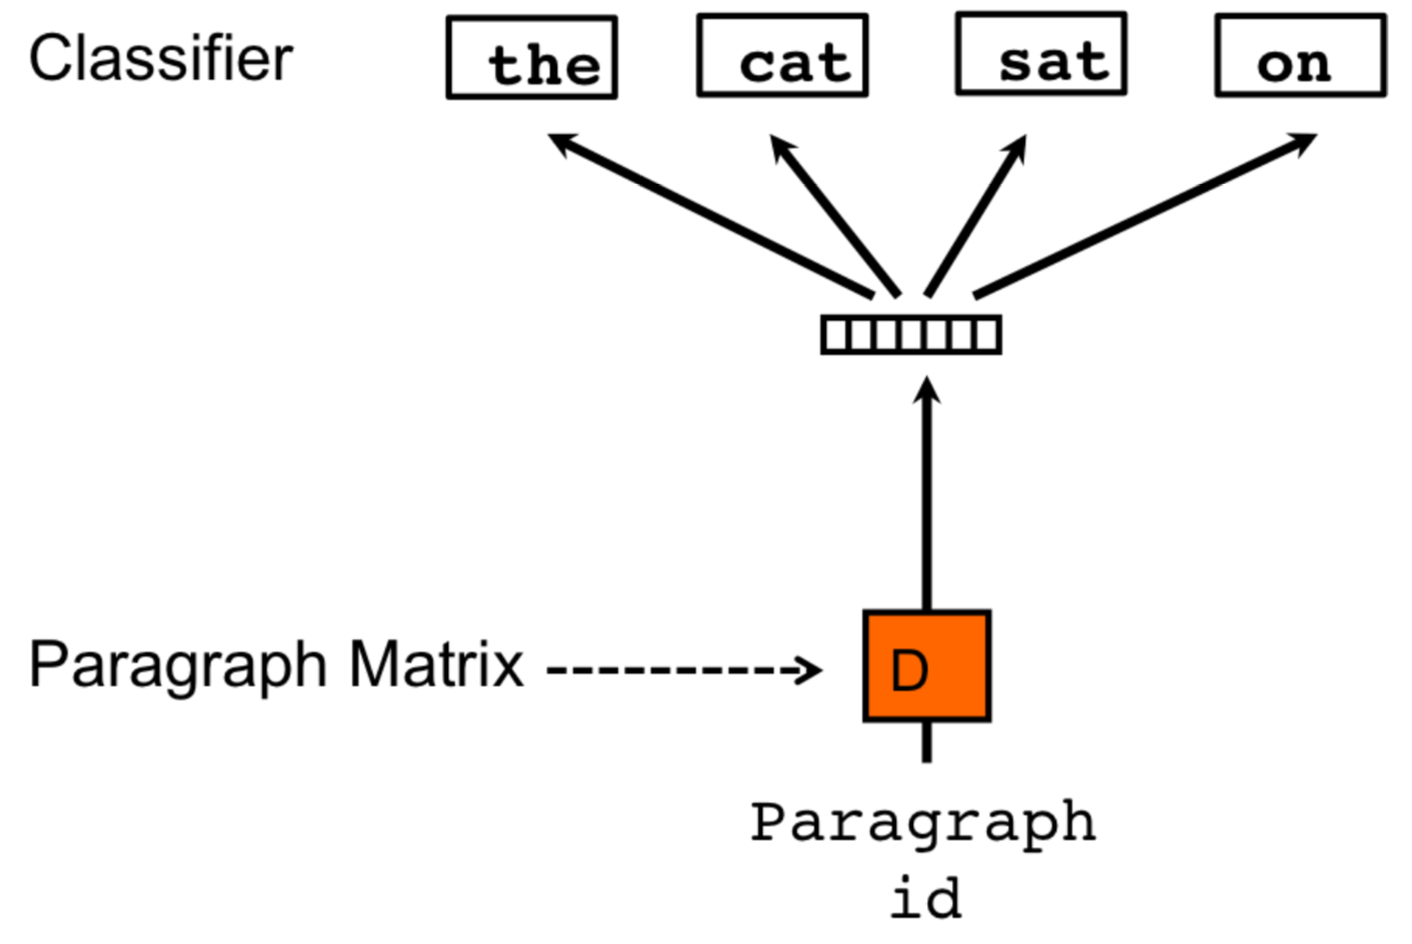
\includegraphics[width=0.3\textwidth]{figures/neural_model_distributed_BOW.png}
				\caption{Distributed BOW model. }
				\label{img:neural_model_distributed_BOW}
			\end{figure}
		\end{itemize}
	\end{itemize}
	\item \textbf{Lexicographical definition}
	\begin{itemize}
		\item We can also use the lexicographical definitions of words to train and/or test the word embeddings
		\item The word embeddings of the definition are combined by an (arithmetic) function $f_c$, and compared to the embedding of the word to be defined
		\item The objective is to minimize the distance to the defined word, but maximize the distance to other words to distinguish between words
		\item An example is shown in Figure~\ref{img:neural_model_lexicographical_definition}
		\begin{figure}[ht]
			\centering
			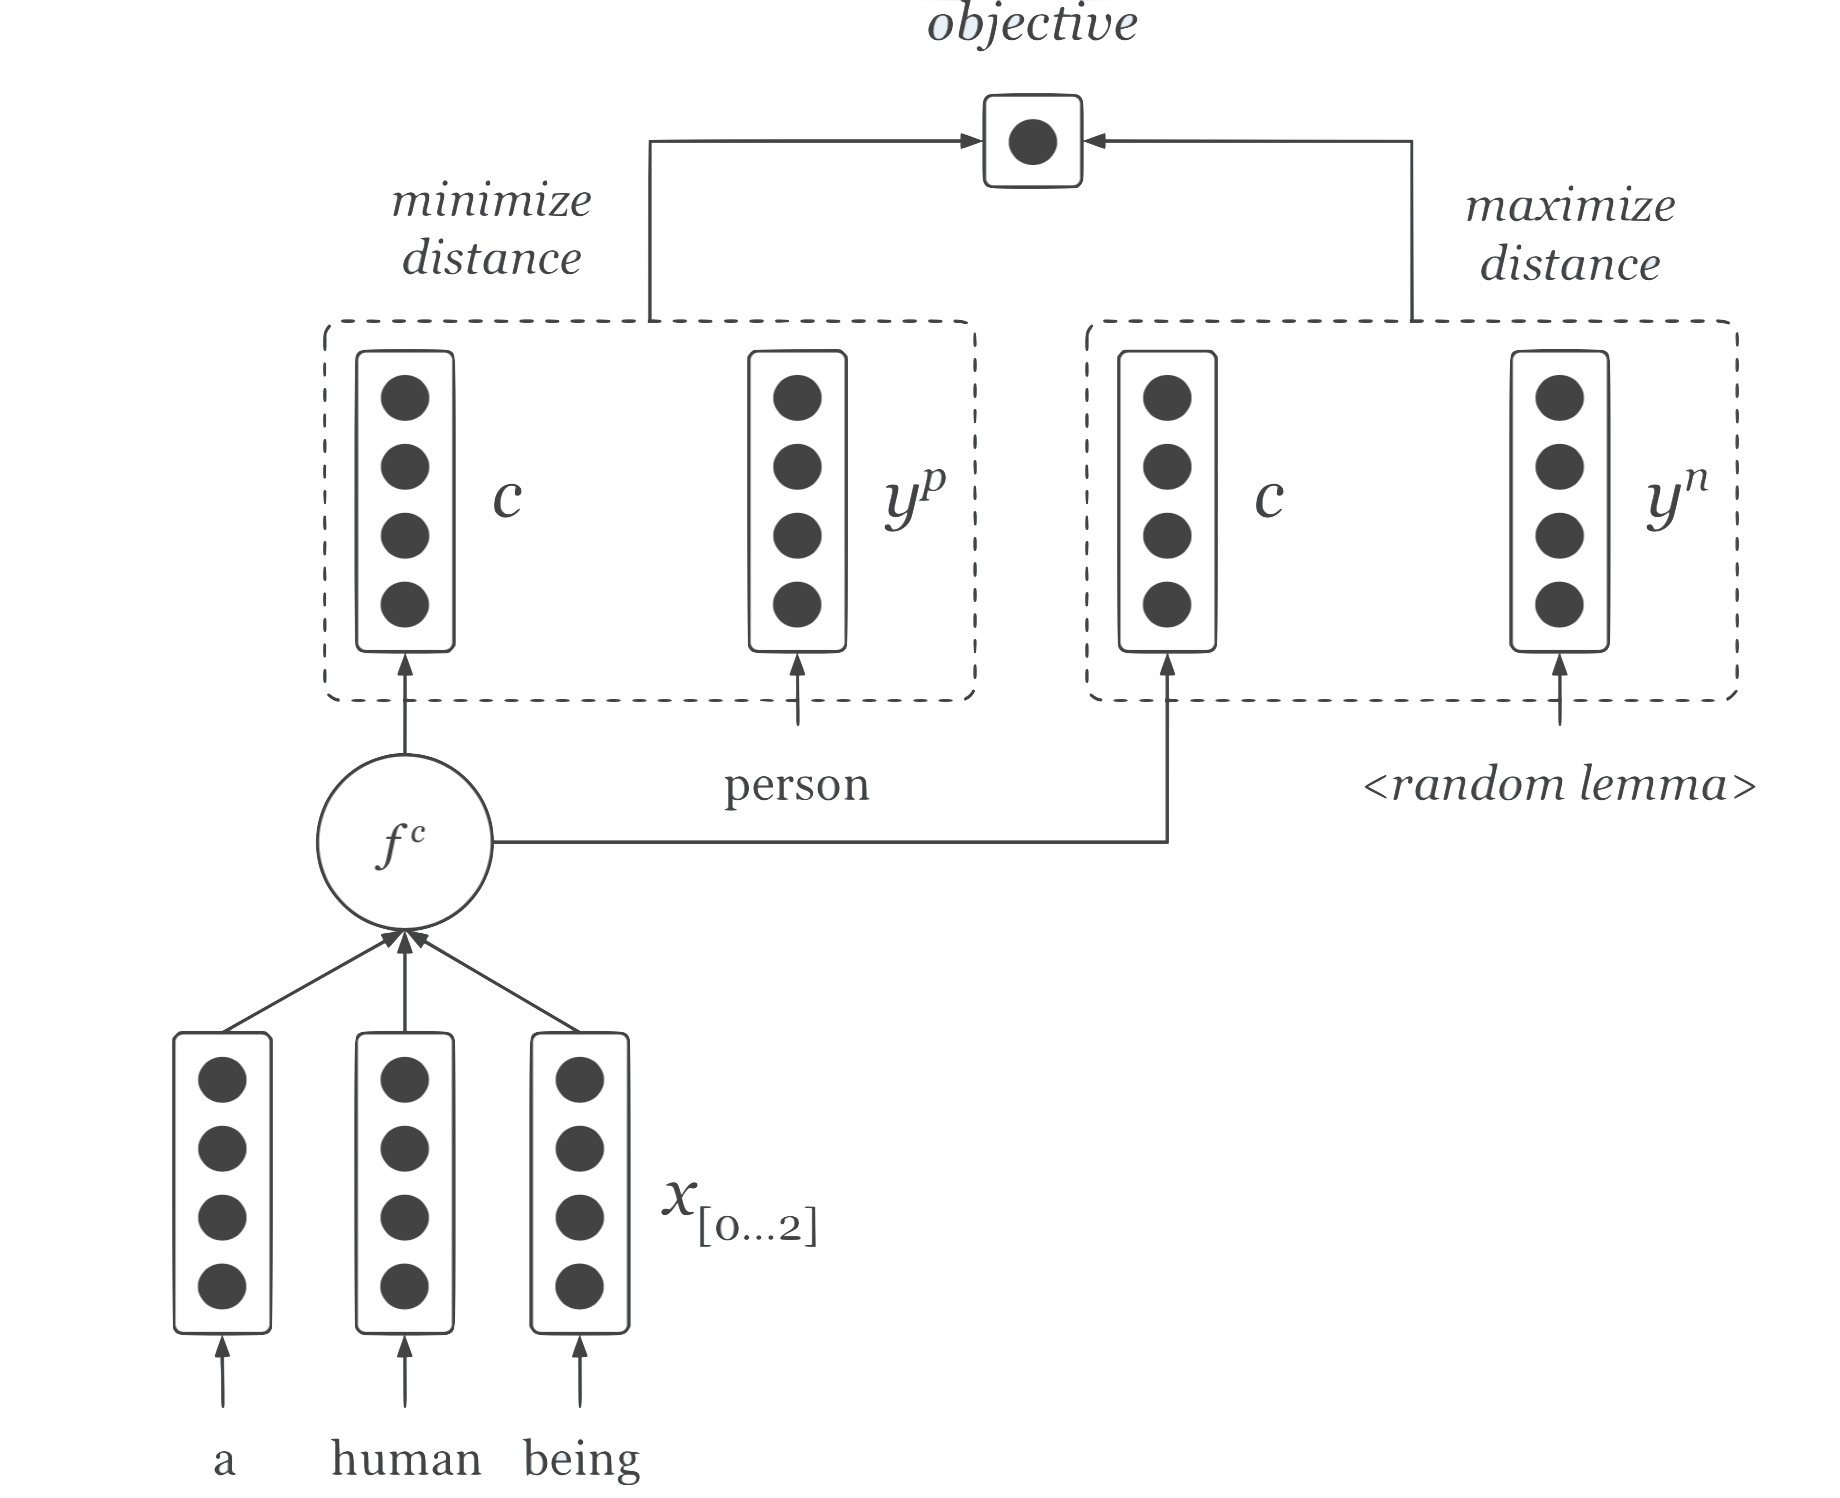
\includegraphics[width=0.3\textwidth]{figures/neural_model_lexicographical_definition.png}
			\caption{Lexicographical model for the example of "\textit{person}" defined as "\textit{a human being}". }
			\label{img:neural_model_lexicographical_definition}
		\end{figure}
	\end{itemize}
\end{itemize}
\subsubsection{Tune word vectors and learn rules of composition}
\begin{itemize}
	\item Deep, neural architectures which have different aspects to be designed
	\item \textbf{Architectures and representation}
	\begin{itemize}
		\item The simplest approach is to use neural networks to embed documents and queries to latent space, and then perform same similarity measures as before (like cosine similarity). This method is also referred to as \textit{Projection to latent space} (see Figure~\ref{img:neural_model_architecture_comparisons_projection_latent_space}). Possible network architectures are Convolutional NN, Recurrent NN or fixed Deep NNs if (max) input size is known
		\item The next step is to replace the similarity measure by another neural network. Thus, this NN takes the composed embeddings of the document and query as input, and return a single real value indicating the similarity score. This approach is called \textit{One Dimensional Matching} and visualized in Figure~\ref{img:neural_model_architecture_comparisons_one_dim_matching}. The common architecture for the highest 
		\item Another architecture is spanning up a two-dimensional input by the query and document. Therefore, we compute similarity scores for every word in the query to every word in the document which results in a two dimensional matrix. On this, we apply a convolutional NN to end up in a fixed-size embedding. A consecutive fully-connected NN maps this embedding into a similarity score. Figure~\ref{img:neural_model_architecture_comparisons_two_dim_matching} visualizes 
	\end{itemize}
	\begin{figure}[ht]
		\centering
		\begin{subfigure}[b]{0.3\textwidth}
			\centering
			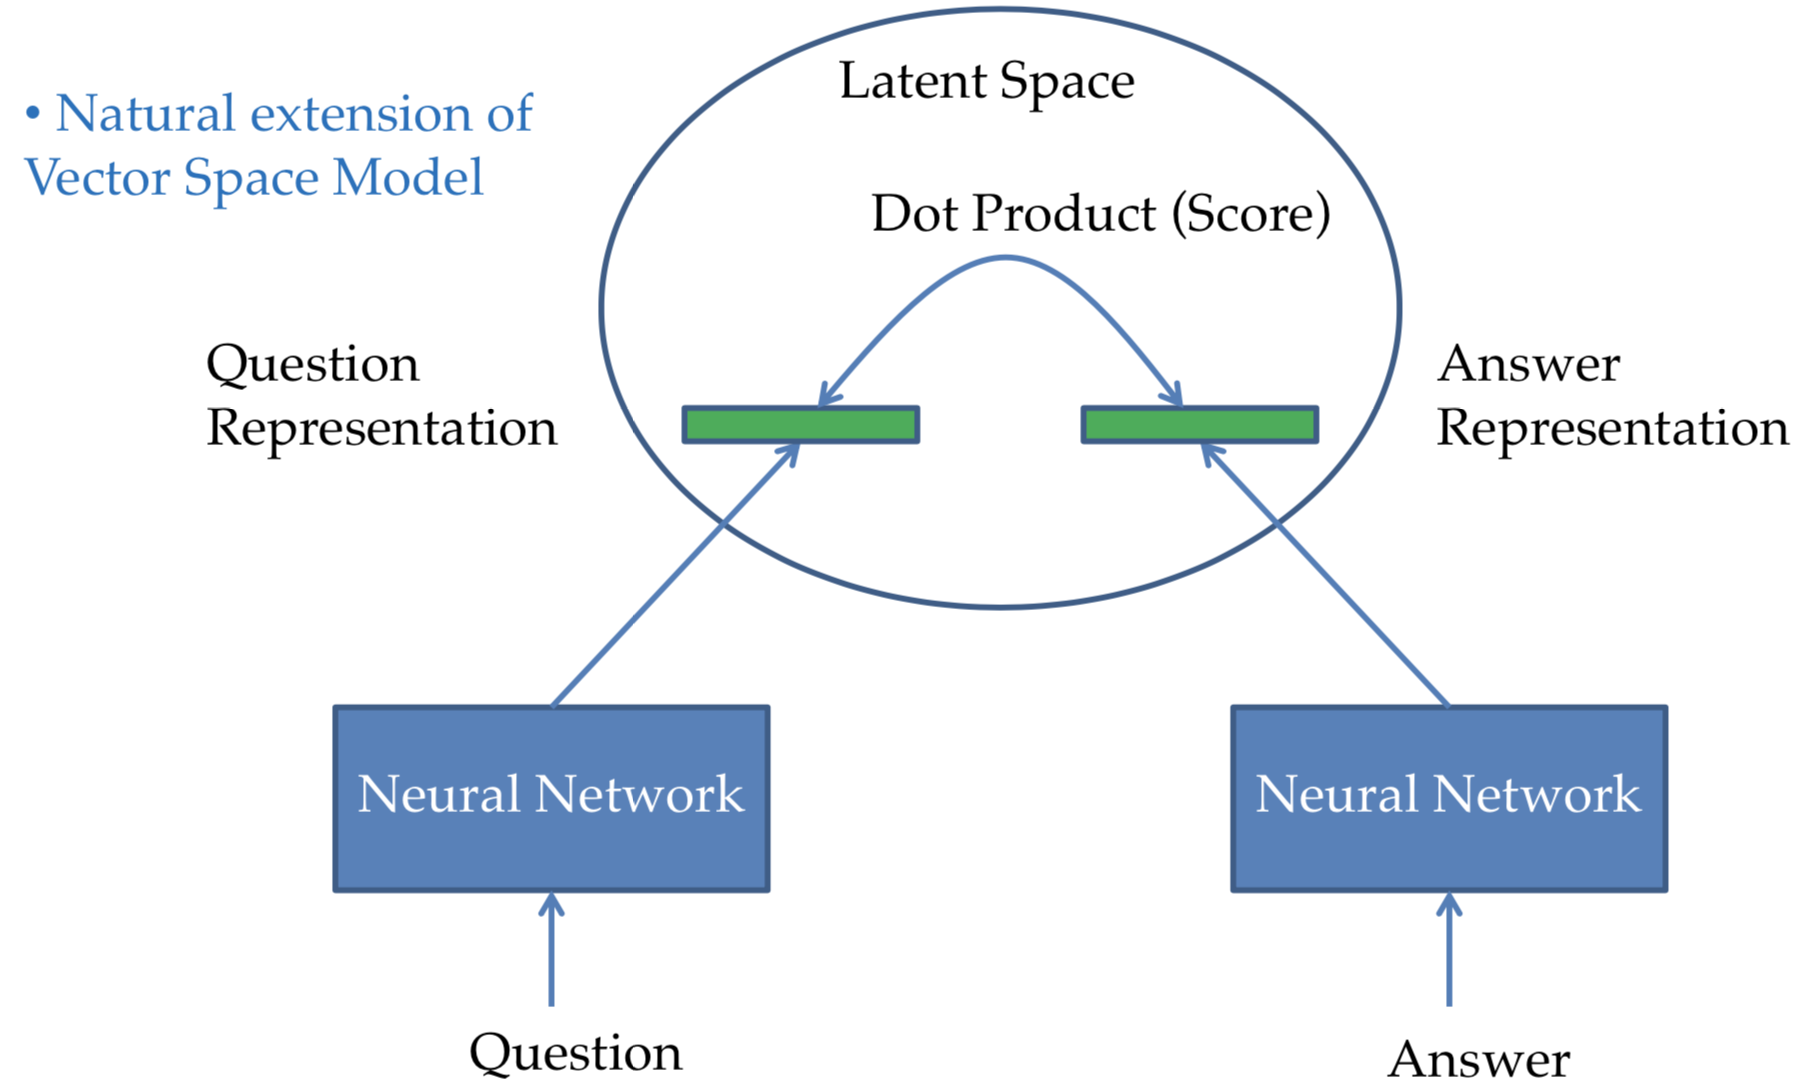
\includegraphics[width=\textwidth]{figures/neural_model_latent_space.png}
			\caption{Projection to Latent space}
			\label{img:neural_model_architecture_comparisons_projection_latent_space}
		\end{subfigure}
		\hspace{2mm}
		\begin{subfigure}[b]{0.3\textwidth}
			\centering
			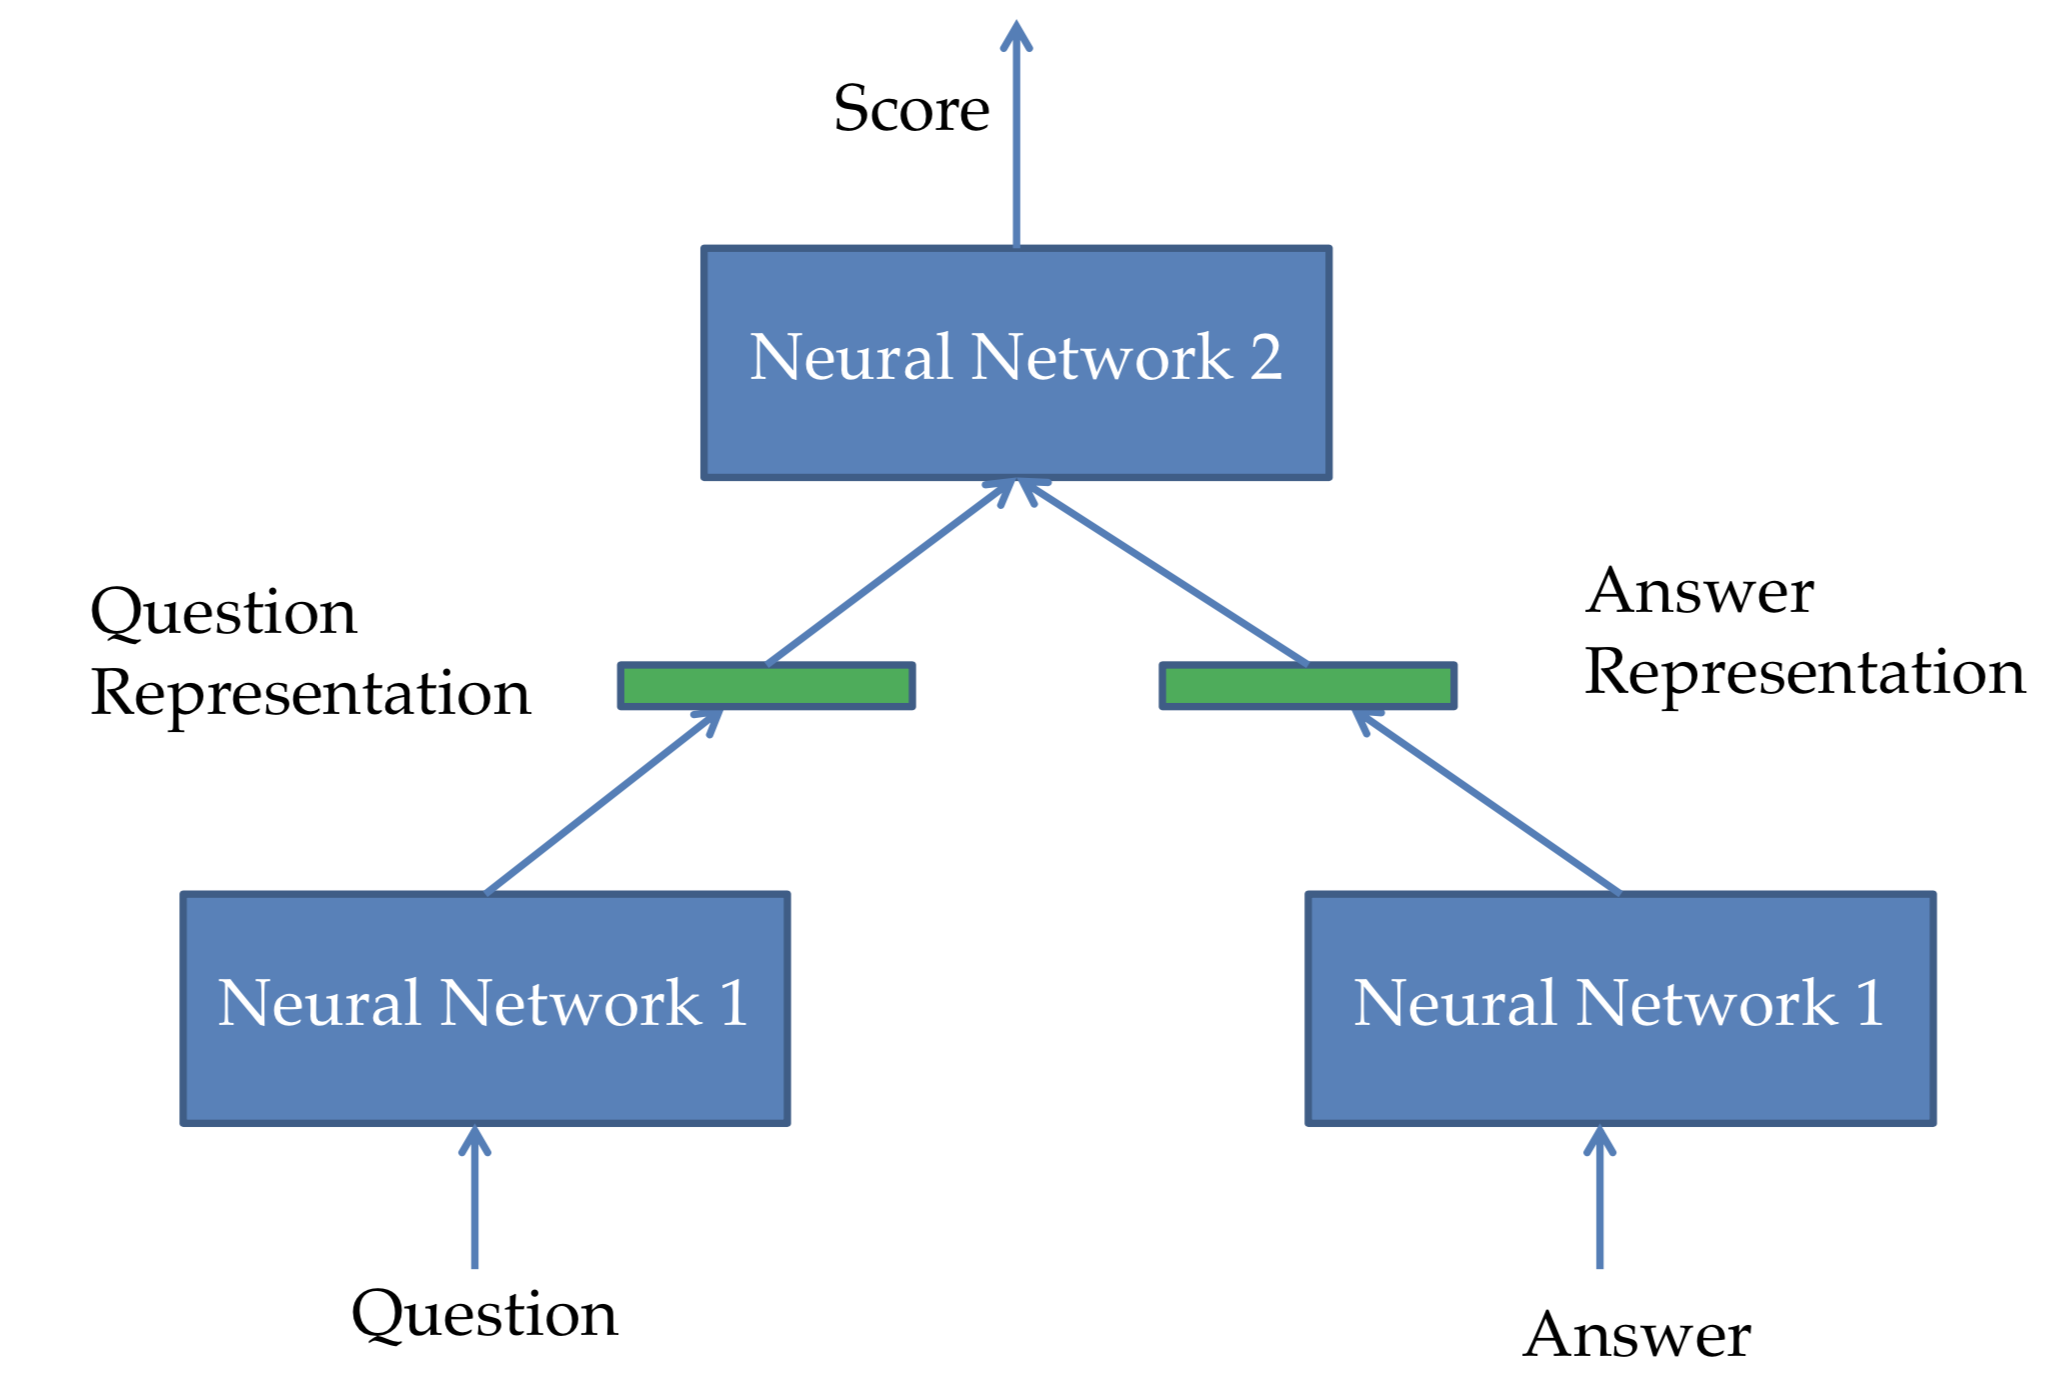
\includegraphics[width=\textwidth]{figures/neural_models_one_dimensional_matching.png}
			\caption{One dimensional matching}
			\label{img:neural_model_architecture_comparisons_one_dim_matching}
		\end{subfigure}
		\hspace{2mm}
		\begin{subfigure}[b]{0.3\textwidth}
			\centering
			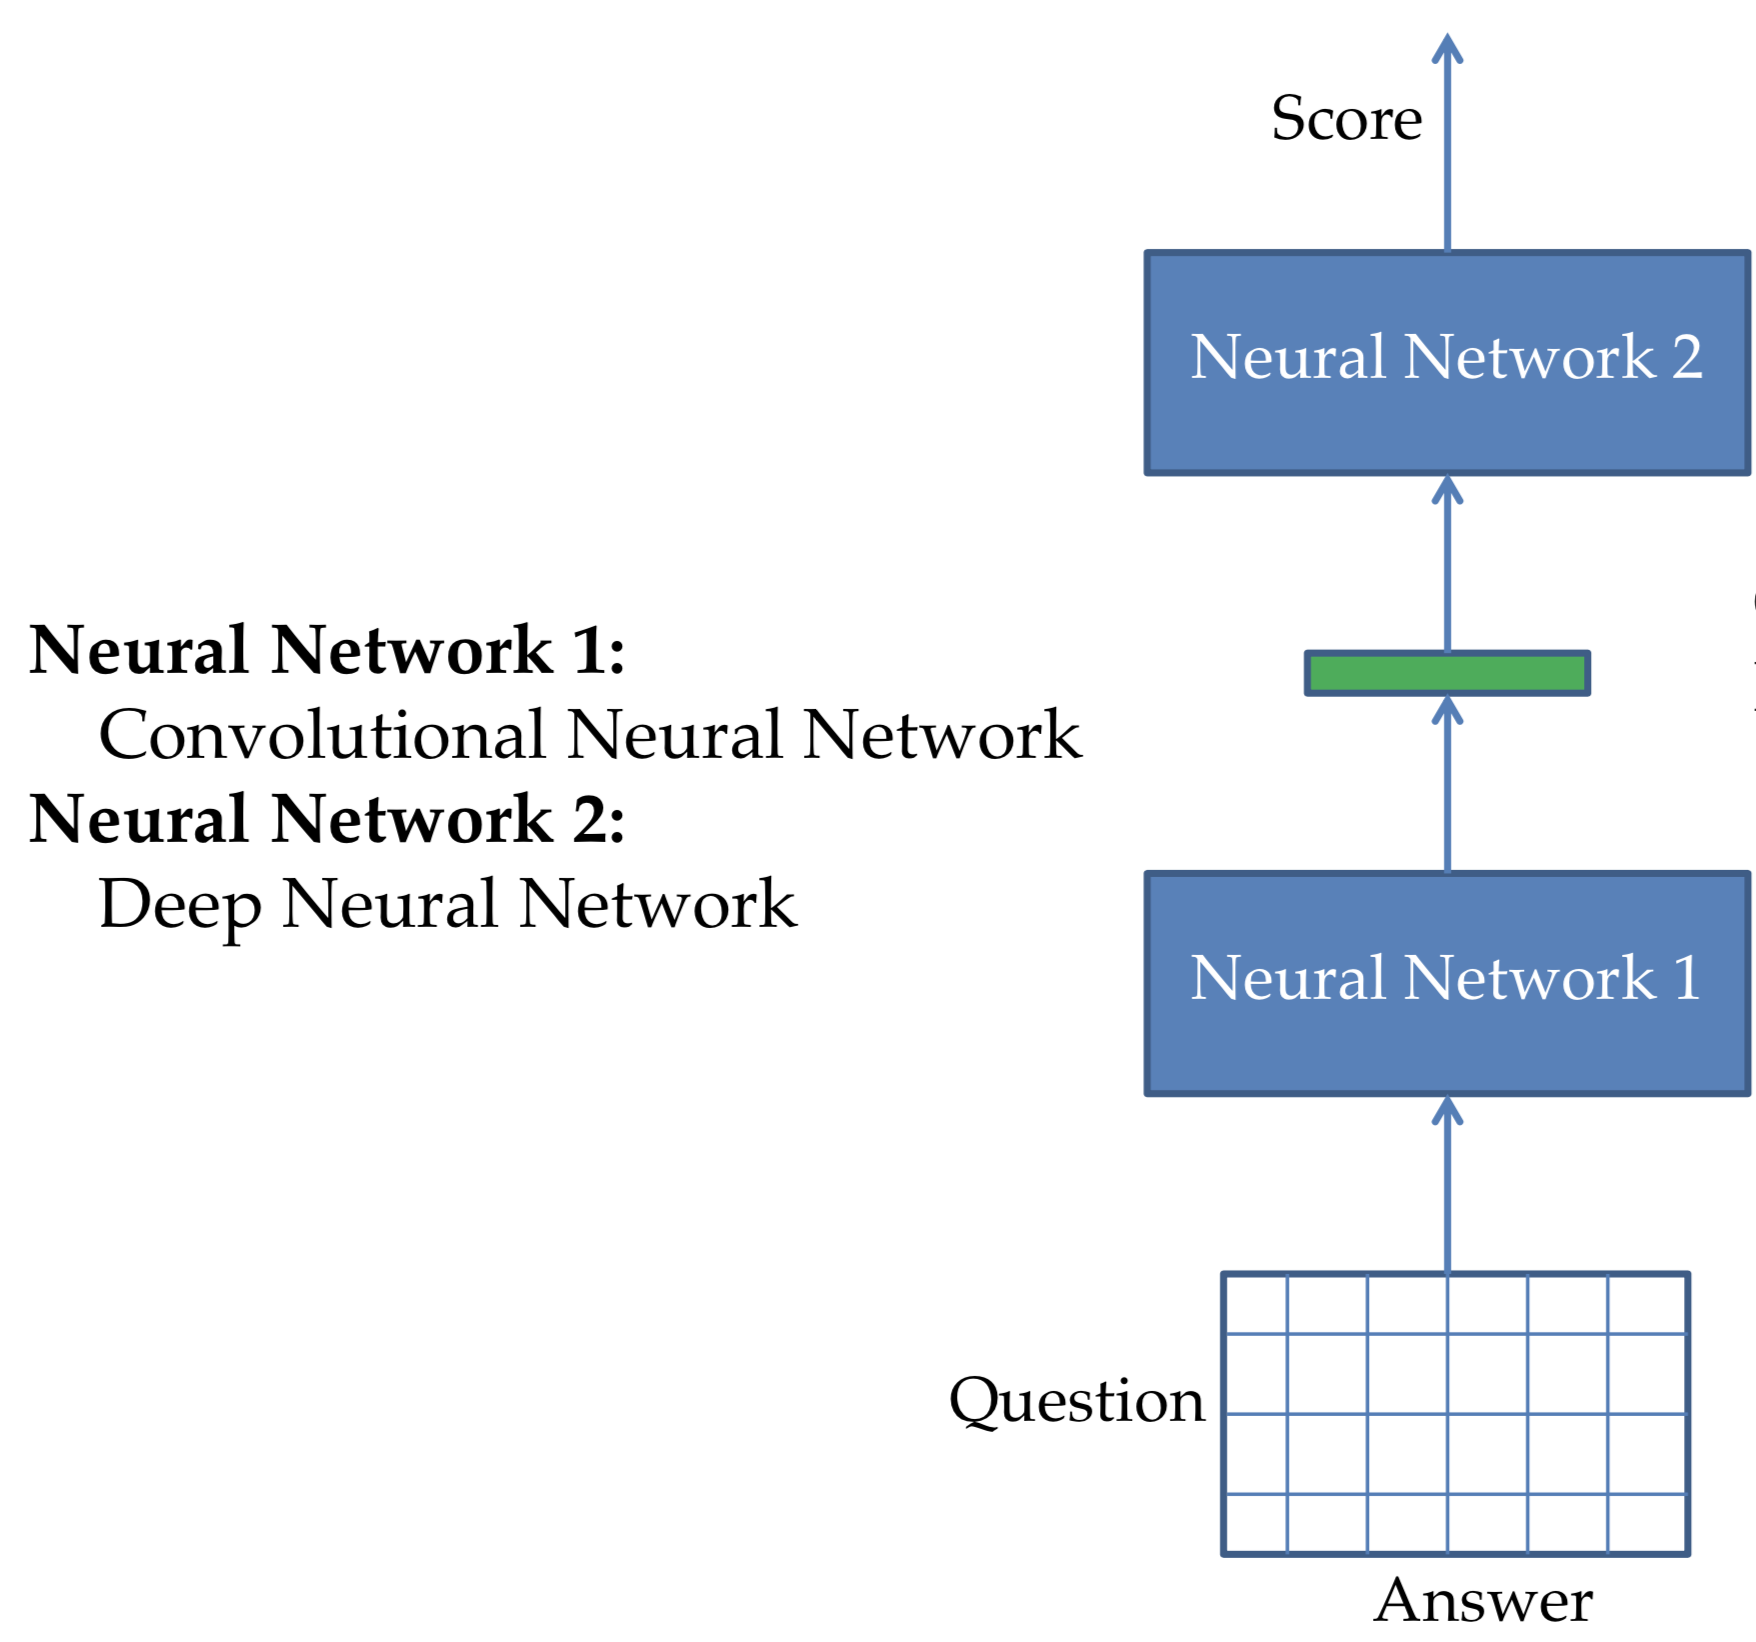
\includegraphics[width=0.8\textwidth]{figures/neural_models_two_dim_matching.png}
			\caption{Two dimensional matching}
			\label{img:neural_model_architecture_comparisons_two_dim_matching}
		\end{subfigure}
		\label{img:neural_model_architecture_comparisons}
		\caption{Comparison of different neural architectures for compositionality}
	\end{figure}
	\item \textbf{Training}: depending on the available data, we can perform different levels of supervision
	\begin{itemize}
		\item \textit{No supervision/labels}: If no labels are provided at all, we could autoencoders to reduce query and document to a latent space and check similarity metrics. Otherwise, we can make use of pretrained neural language models with techniques like ELMo and BERT
		\item \textit{Distant supervision}: We create pseudo-labels by sampling short word sequences from a document and considering this as query. The document from which we sampled is labeled as relevant/high similarity, while all other documents (from which we sample one randomly for training) are considered as being not relevant
		\item \textit{Weak supervision}: As alternative, we can use unsupervised ranking functions like BM25 to generate labels and use this scores for training (teacher-student architecture). In experiments, the neural network was even able to outperform BM25.
		\item \textit{Full supervision}: Labels are created by either annotators or using the click log as implicit feedback from the users. We can train the models in a standard supervised fashion. 
	\end{itemize}
\end{itemize}